%\newpage
\section{Widerstands-Messung}
Jeder Widerstand wird mit vier verschiedenen Messmethoden in einer Stromrichtung vermessen.
Der gleiche Widerstand wird auch mit den gleichen vier Messmethoden in die andere Stromrichtung vermessen.
Die Messung in die Gegenrichtung wird nur für die Erkennung auf Widerstand benutzt.
Wenn die Abweichung dieser beiden Messungen zu groß ist, ist es kein Widerstand.

\subsection{Widerstandsmessung mit den 680-Ohm-Widerständen}
Die Messung des unbekannten Widerstandes Rx wird in zwei verschiedenen Wegen mit den \(680\Omega\)-Präzisionswiderständen
 durchgeführt.
Das Schaltbild dieser Messungen mit Testpin 1 (TP1) und Testpin 3 (TP3) werden vereinfacht in Abbildung~\ref{fig:RL1mes} und Abbildung~\ref{fig:RL2mes} als ein Beispiel von den sechs Kombinationsmöglichkeiten gezeigt.

\begin{figure}[H]
\centering
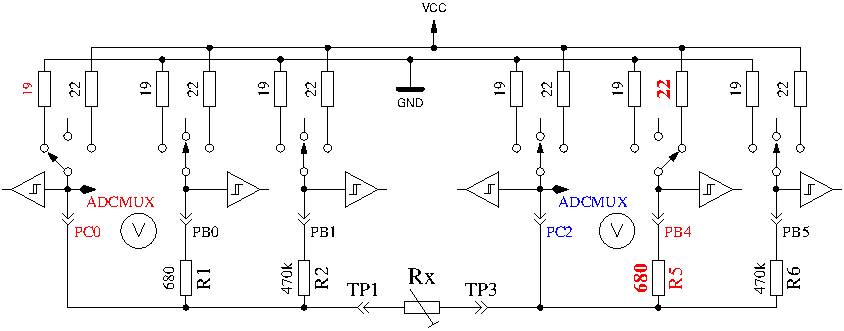
\includegraphics[]{../FIG/ResistormessL1.pdf}
\caption{Messung Type 1 mit \(680\Omega\) }
\label{fig:RL1mes}
\end{figure}

\begin{figure}[H]
 \centering
 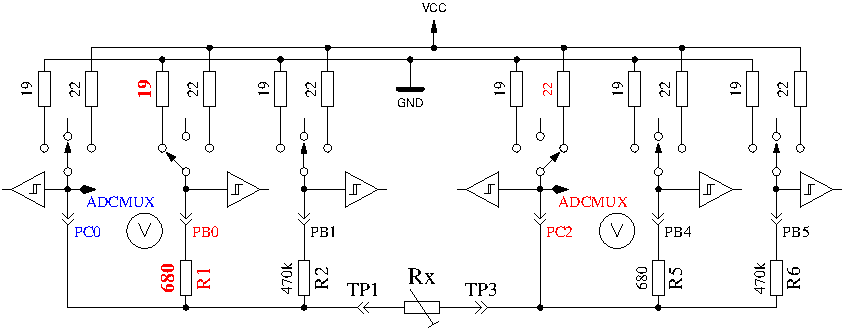
\includegraphics[]{../FIG/ResistormessL2.pdf}
 \caption{Messung Type 2 mit \(680\Omega\) }
\label{fig:RL2mes}
\end{figure}

Auf der linken Seite wird der Testpin 1 und auf der rechten Seite der Testpin 3 gezeigt.
In beiden Schaltungen kann man erkennen, dass der Anschluss 3 (TP3) mit VCC und die linke Seite (TP1) mit
GND verbunden ist.
Die Stromrichtung durch den Widerstand Rx ist immer die gleiche.
Die Werte für auf Ausgang geschaltete Ports werden mit roter Farbe dargestellt, 
die Werte für die Eingänge werden mit blauer Farbe dargestellt, inaktive Ports sind schwarz.
In beiden gezeigten Messmethoden sollte der Strom den gleichen Wert haben, weil die Summe der Widerstände zwischen
VCC und GND gleich ist, vorausgesetzt die eingebauten Widerstände sind gleich.
Normalerweise sind die gemessenen Spannungen aber nicht gleich, weil die Reihenfolge
der Widerstände vertauscht ist.

Das V-Symbol innerhalb eines Kreises markiert die Ports, die für die Spannungsmessung benutzt werden.
In beiden Konfigurationen kann der Wert des Widerstandes Rx aus den bekannten Widerstandswerten
und den gemessenen Spannungen berechnet werden, wenn das Verhältnis des Widerstands Rx und den \(680\Omega\)-Widerständen
 nicht zu hoch ist.
Der theoretische Spannungsverlauf wird in Abbildung~\ref{fig:RLvtot} gezeigt, wobei die Widerstandswerte 
in logarithmischer Skalierung dargestellt sind.
\begin{figure}[H]
\centering
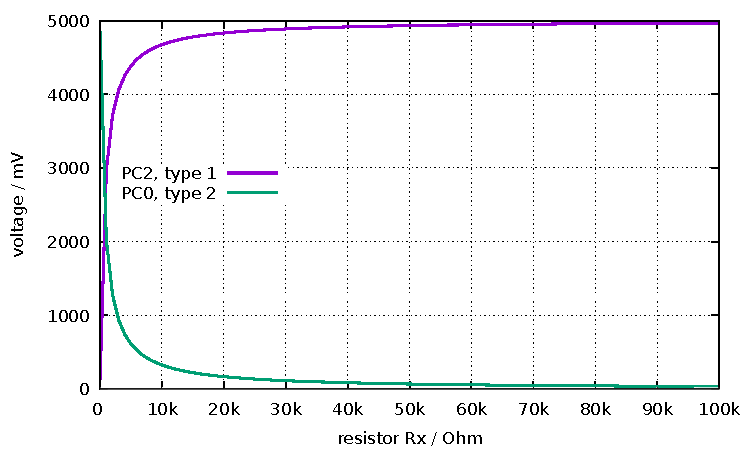
\includegraphics[width=16cm]{../GNU/RLvtot.pdf}
\caption{Spannung von Type 1 und Type 2 mit Messwiderstand \(680\Omega\) }
\label{fig:RLvtot}
\end{figure}
Die Verlauf für Messung Type 1 wird in Abbildung~\ref{fig:RLvlow} mit gespreizter Darstellung für die unteren Widerstandwerte gezeigt.
Wie man sehen kann, braucht man eine bessere ADC-Auflösung als die möglichen \(4,9mV\) bei der \(5V\) ADC-Referenz, um richtige
Widerstandswerte von der gemessenen Spannung unter \(2\Omega\) zu erhalten.
Es gibt nur drei ADC-Stufen mit der \(5V\)-Referenz zwischen \(0\Omega\) und \(2\Omega\).
Hier kann die Bereichsumschaltung mit der AUTOSCALE\_ADC-Option helfen.
Der gleiche gespreizte Bereich für die Type-2-Messung wird in Abbildung~\ref{fig:RLvhigh} gezeigt.
Unglücklicherweise kann man nicht die höhere ADC-Auflösung für Messmethode Type 2 benutzen,
weil die Spannung zu hoch ist und unser ATmega keine differentiellen ADC-Eingänge besitzt.
Die Messungen mit den \(680\Omega\)-Widerständen werden bis zu einem Widerstandswert von 
\(20k\Omega\) (Spannung ist unter \(169mV\)) zur Bestimmung des Messergebnisses verwendet.

Für höhere Widerstandswerte werden Messungen mit den \(470k\Omega\)-Widerständen benutzt.
Der Mittelwert von beiden Messungen wird für den angezeigten Widerstandwert benutzt, wenn alle Messungen ergeben,
dass es kein anderes Bauteil ist.
Wenn die AUTOSCALE\_ADC-Funktion benutzt wird und eine der gemessenen Spannungen für beide Versionen unter 0,98V liegt,
wird ein gewichteter Mittelwert mit Faktor Vier für die Messung mit der Spannung unter \(0,98V\) benutzt. Der andere Wert wird mit Faktor Eins bewertet.
Das wird wegen der Faktor Vier besseren Auflösung dieser Messung gemacht.
Faktor Vier wird nur für ATmega168- und ATmega328-Prozessoren verwendet, für ATmega8 wird ein
Faktor Zwei als Wichtung benutzt wenn die Spannung unter \(0,98V\) ist, weil die ADC-Referenzspannung hier \(2,56V\) statt \(1,1V\) beträgt.
Wenn der ATmega mehr als 8 KByte Flashspeicher besitzt, wird die Spannungsmessung an den Widerständen so lange verzögert,
bis keine Änderung mehr festgestellt wird oder eine Zeitgrenze überschritten wird.
Durch diese Maßnahme werden auch große Kondensatoren nicht mehr irrtümlich als
Widerstände erkannt und der Gleichstrom-Widerstand großer Induktivitäten wird richtig gemessen.

\begin{figure}[H]
  \begin{subfigure}[b]{9cm}
    \centering
    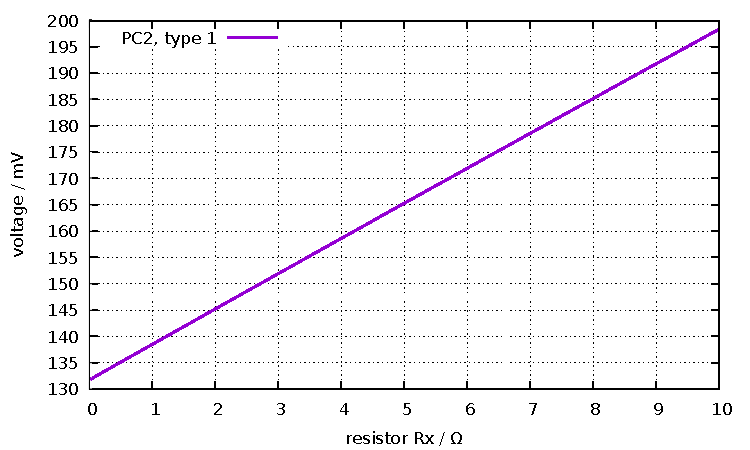
\includegraphics[width=9cm]{../GNU/RLvlow.pdf}
    \caption{Type 1 Messung}
    \label{fig:RLvlow}
  \end{subfigure}
  ~
  \begin{subfigure}[b]{9cm}
    \centering
    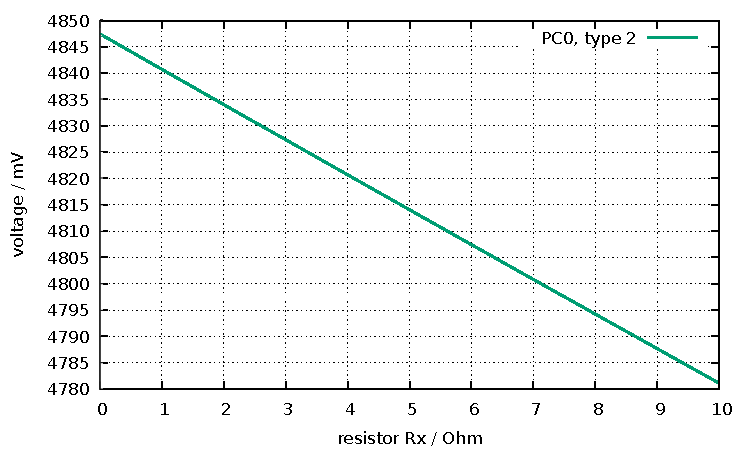
\includegraphics[width=9cm]{../GNU/RLvhigh.pdf}
    \caption{Type 2 Messung}
    \label{fig:RLvhigh}
  \end{subfigure}
  \caption{Ausschnitt des theoretischen Spannungsverlauf von \(0\Omega\) bis \(10\Omega\)}
\end{figure}


\subsection{Widerstandsmessung mit den 470-kOhm-Widerständen}
Die nächsten Abbildungen~\ref{fig:RH1mes} und \ref{fig:RH2mes} zeigen die gleichen Messmethoden für die Messungen mit
 \(470k\Omega\)-Präzisionswiderständen.
Weil \(470k\Omega\) in Relation zu den Port-Widerständen \(22\Omega\) und \(19\Omega\) sehr groß ist,
können die Port-Widerstände für die Berechnung des Widerstandswertes Rx vernachlässigt werden.

Für beide Messmethoden mit den \(470k\Omega\)-Widerständen wird nur eine Spannung gemessen, weil der Strom
so niedrig ist, dass keine Spannungsdifferenz an den internen Port Widerständen gemessen werden kann (wie zu erwarten).
Der theoretische Spannungsverlauf wird in Abbildung~\ref{fig:RHv} gezeigt, wobei die Widerstandswerte wieder in
logarithmischer Skalierung gezeigt werden.
Der theoretische Verlauf in diesem Diagramm endet bei \(100M\Omega\), aber das Ergebnis des Testers wird auf
 \(60M\Omega\) begrenzt, anderenfalls nimmt der Tester an, dass kein Widerstand angeschlossen ist.
Als Ergebnis wird der gewichtete Mittelwert von beiden Messmethoden verwendet. Dies geschieht nach den gleichen Regeln, die schon bei
den Messungen mit den  \(680\Omega\) Widerständen beschrieben wurden.
Ich habe beobachtet, dass die Messergebnisse für alle ATmega-Typen  näher am wahren Wert liegen, wenn zum Messergebnis
ein konstanter Offset von \(350\Omega\) addiert wird.
Dieser Offset kann mit der Konstante RH\_OFFSET (define) in der Datei config.h angepasst werden.

\begin{figure}[H]
\centering
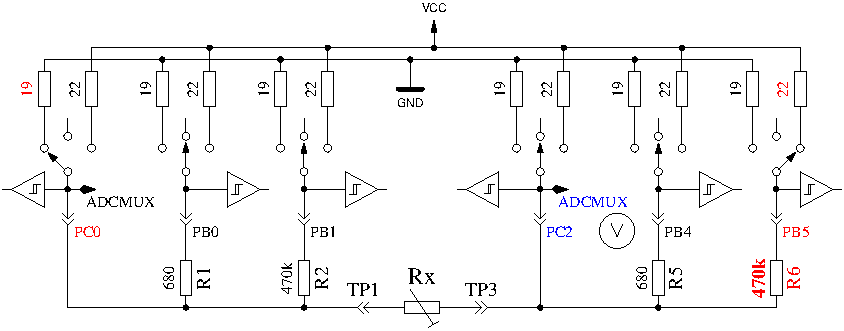
\includegraphics[]{../FIG/ResistormessH1.pdf}
\caption{Messung Type 3 mit \(470k\Omega\) }
\label{fig:RH1mes}
\end{figure}

\begin{figure}[H]
 \centering
 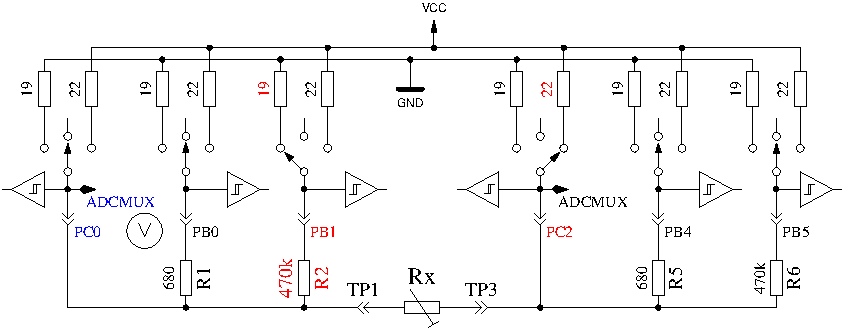
\includegraphics[]{../FIG/ResistormessH2.pdf}
 \caption{Messung Type 4 mit \(470k\Omega\) }
\label{fig:RH2mes}
\end{figure}

\begin{figure}[H]
\centering
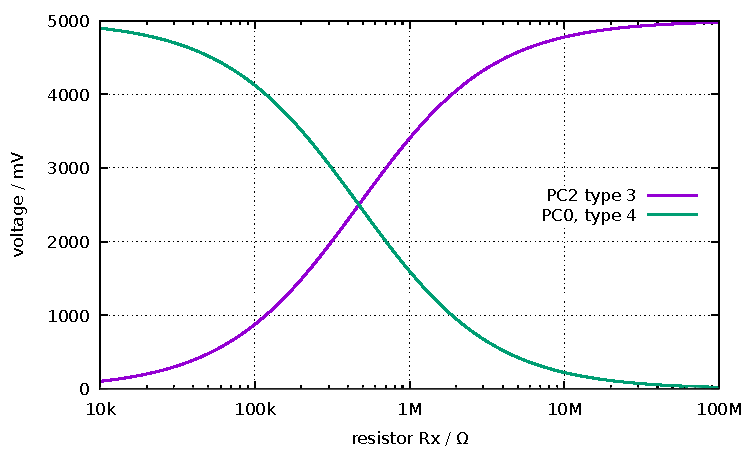
\includegraphics[width=16cm]{../GNU/RHv.pdf}
\caption{Spannungen bei Messungen von Type 3 und Type 4  mit \(470k\Omega\) }
\label{fig:RHv}
\end{figure}

\subsection{Ergebnisse der Widerstands-Messung}
Abbildung~\ref{fig:mega8res} zeigt den relativen Fehler der Widerstandmessung mit drei verschiedenen ATmega8. 
Zusätzlich werden die Messergebnisse einiger Widerstände mit der Originalsoftware von Markus F. als
,,Mega8orig'' gezeigt.
Die Messergebnisse der gleichen Widerstände mit je drei ATmega8A und drei ATmega8L werden in den Abbildungen
\ref{fig:mega8Ares} und \ref{fig:mega8Lres} gezeigt.
Abbildung~\ref{fig:mega168res} zeigt die gleichen Messungen mit einem ATmega168.
,,Mega168'' sind die Ergebnisse ohne die AUTOSCALE\_ADC Option, ,,Mega168as'' die mit der
 AUTOSCALE\_ADC-Option.

Mit dem ATmega168 scheint es möglich zu sein, Messungen von Widerständen im
Bereich von \(20\Omega\) bis \(20M\Omega\) mit einem Messfehler von unter \(\pm1\%\) durchzuführen.
Für Messungen unterhalb von \(100\Omega\) sollte man berücksichtigen, dass jede Prüfklemme mit Kabel ebenfalls
einen Widerstandwert hat.
Es ist besser, den Widerstand direkt mit den Anschlussklemmen zu verbinden.
Wenn das nicht möglich ist, sollte man der Widerstandswert der kurzgeschlossenen Prüfklemmen vom Messergebnis abziehen.
Zeigt beispielsweise der Tester einen Wert von \(30,6\Omega\) an, wenn der Präzisionswiderstand einen aufgedruckten Wert von \(30\Omega\) hat, 
und die im Kurzschluss gemessenen Prüfklemmen haben einen Wert von \(0,5\Omega\), dann wird der Widerstand vom
Tester mit \(30,1\Omega\) gemessen.
Unterhalb von einem Widerstandswert von \(10\Omega\) macht ein Auflösungs-Schritt von \(0,1\Omega\) schon einen Fehler von mehr als \(1\%\)!

\begin{figure}[H]
\centering
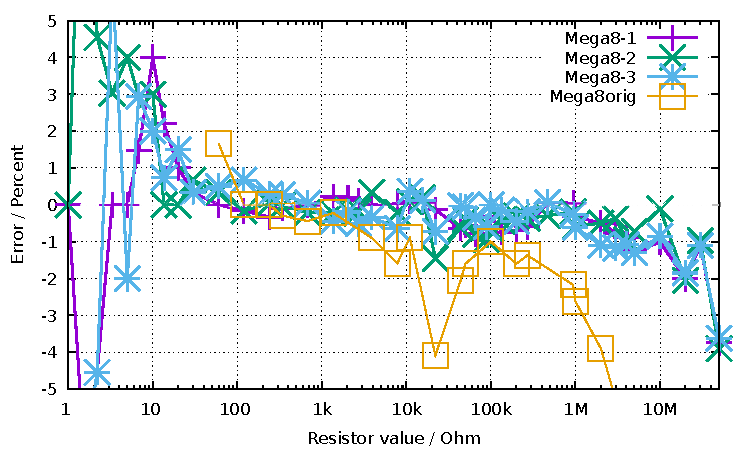
\includegraphics[width=16cm]{../GNU/Mega8res.pdf}
\caption{Relativer Fehler für Widerstands-Messungen mit ATmega8 }
\label{fig:mega8res}
\end{figure}

\begin{figure}[H]
  \begin{subfigure}[b]{9cm}
    \centering
    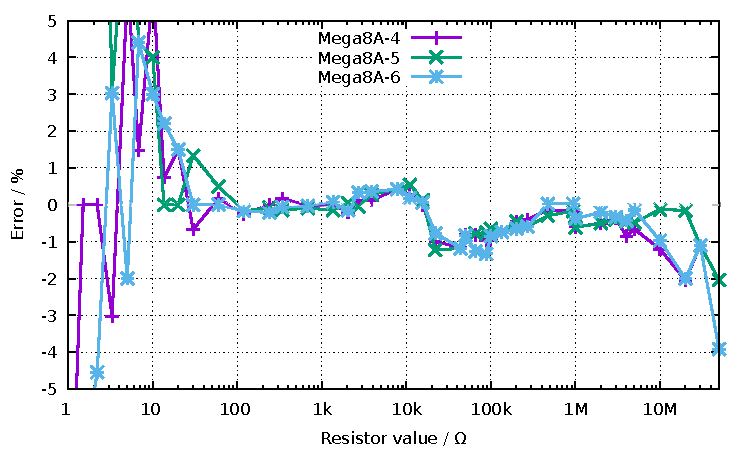
\includegraphics[width=9cm]{../GNU/Mega8Ares.pdf}
    \caption{mit drei ATmega8A}
    \label{fig:mega8Ares}
  \end{subfigure}
  ~
  \begin{subfigure}[b]{9cm}
    \centering
    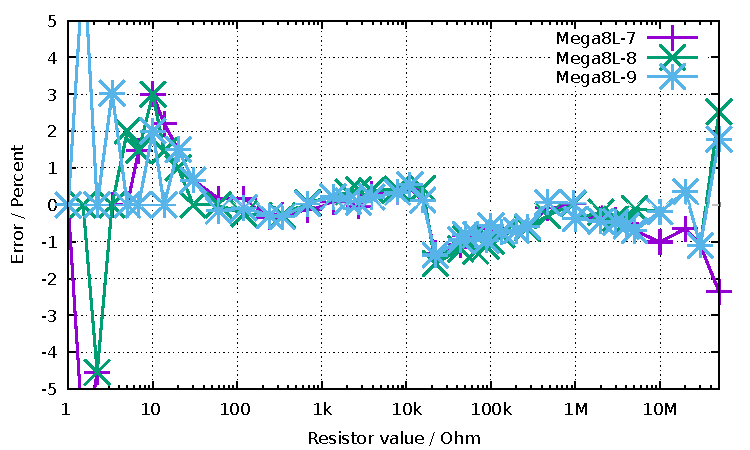
\includegraphics[width=9cm]{../GNU/Mega8Lres.pdf}
    \caption{mit drei ATmega8L}
    \label{fig:mega8Lres}
  \end{subfigure}
\caption{Relativer Fehler für Widerstands-Messungen}
\end{figure}

\begin{figure}[H]
\centering
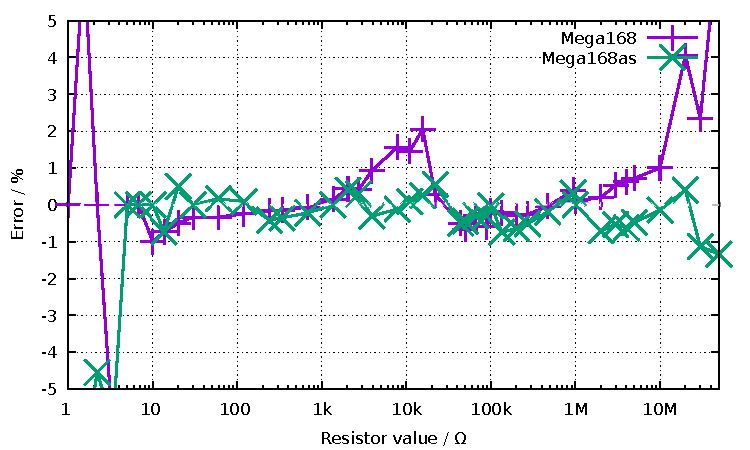
\includegraphics[width=16cm]{../GNU/Mega168res.pdf}
\caption{Relativer Fehler für Widerstand-Messungen mit ATmega168 }
\label{fig:mega168res}
\end{figure}

Das Diagramm \ref{fig:m168res_all} zeigt die Messfehler von drei ATmega168-Prozessoren vor der Kalibration als Punkte, nach der
Kalibration als Linie. Entsprechend werden die Messfehler von drei ATmega168A in Abbildung \ref{fig:m168ares_all} und
die Messfehler von drei ATmega328P in Abbildung \ref{fig:m168pres_all} gezeigt.
Die Messfehler der ATmega328 werden in den Abbildungen \ref{fig:m328res_all} und \ref{fig:m328pres_all} gezeigt.
Nach der automatischen Kalibration bleibt der Messfehler mit einer Ausnahme (ATmega328P-13, \(22k\Omega\)) im Widerstandsbereich
\(10\Omega~-~20M\Omega\) im Bereich \(\pm1\%\).
Vor der Kalibration können die Messfehler bei einigen Prozessoren bis \(\pm~3\%\) betragen.
Der Fehler wird verursacht durch die AUTOSCALE\_ADC-Umschaltung der ADC-Referenz.
Durch den direkten Vergleich einer Kondensatorspannung von unter \(1V\), einmal mit der VCC-Referenz und nochmal mit
der internen ADC-Referenz gemessen, kann der Fehler ausgeglichen werden.
In diesem Fall wird die Spannung mit dem gleichen Multiplexer-Kanal gemessen und die Bandgap-Referenz ist auf den AREF-Pin
aufgeschaltet.
Die direkte Vermessung der Bandgap-Referenz durch die direkte Wahl des Multiplexer-Eingangs führt leider zu diesem Offset,
der entweder manuell mit der Option REF\_R\_KORR oder automatisch mit der Option AUTO\_CAL des Selbsttestes beseitigt werden kann.
Im AUTO\_CAL-Modus ist REF\_R\_KORR ein zusätzlicher Offset zur automatisch gefundenen Spannungsdifferenz.

\begin{figure}[H]
  \begin{subfigure}[b]{9cm}
    \centering
    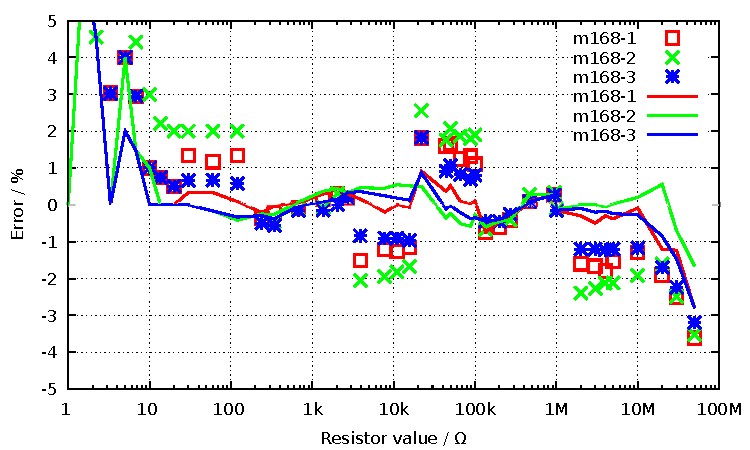
\includegraphics[width=9cm]{../GNU/m168res_all.pdf}
    \caption{mit drei ATmega168}
    \label{fig:m168res_all}
  \end{subfigure}
  ~
  \begin{subfigure}[b]{9cm}
    \centering
    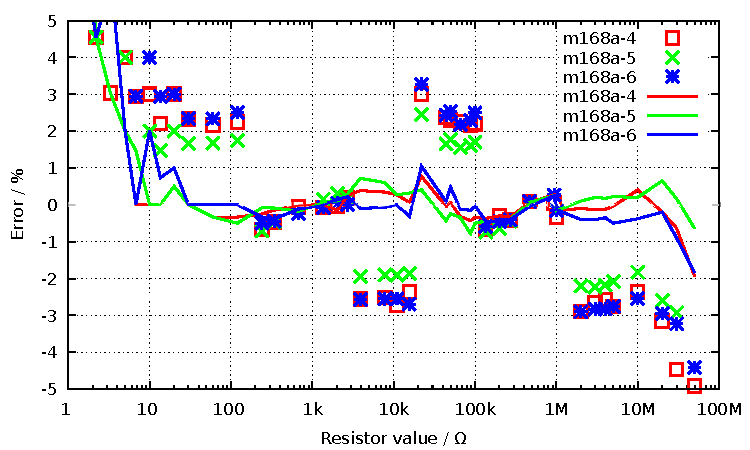
\includegraphics[width=9cm]{../GNU/m168ares_all.pdf}
    \caption{mit drei ATmega168A}
    \label{fig:m168ares_all}
  \end{subfigure}
\caption{Relativer Fehler für Widerstands-Messungen}
\end{figure}

\begin{figure}[H]
\centering
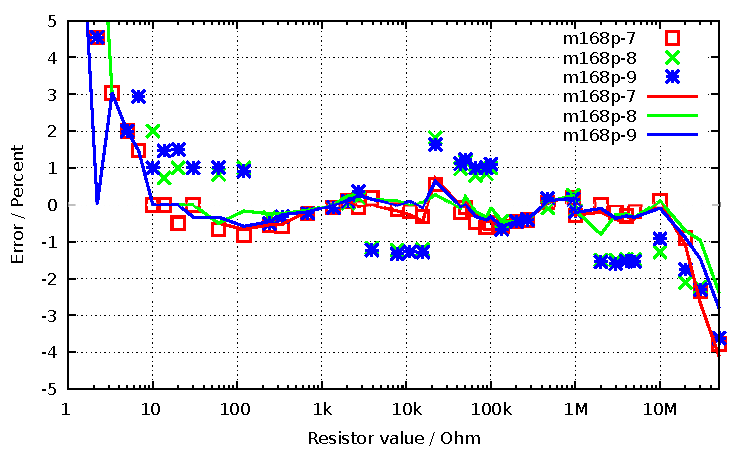
\includegraphics[width=16cm]{../GNU/m168pres_all.pdf}
\caption{Relativer Fehler für Widerstands-Messungen mit drei ATmega168P }
\label{fig:m168pres_all}
\end{figure}

\begin{figure}[H]
  \begin{subfigure}[b]{9cm}
    \centering
    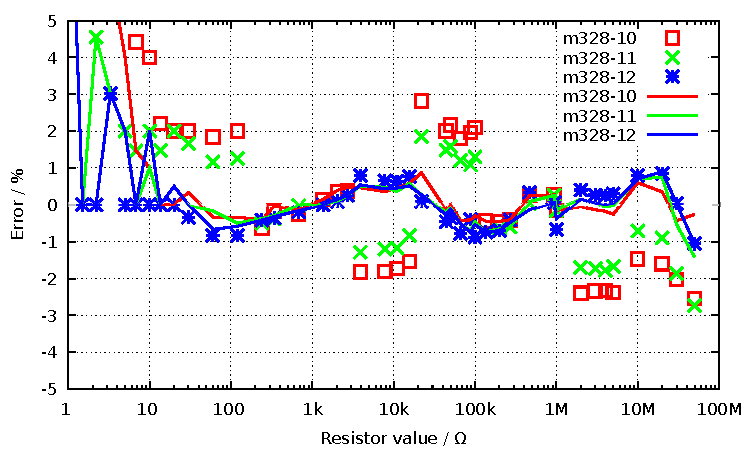
\includegraphics[width=9cm]{../GNU/m328res_all.pdf}
    \caption{mit drei ATmega328}
    \label{fig:m328res_all}
  \end{subfigure}
  ~
  \begin{subfigure}[b]{9cm}
    \centering
    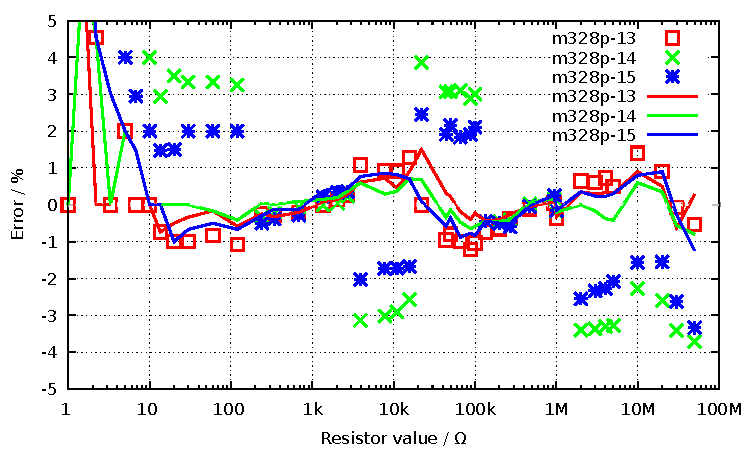
\includegraphics[width=9cm]{../GNU/m328pres_all.pdf}
    \caption{mit drei ATmega328P}
    \label{fig:m328pres_all}
  \end{subfigure}
\caption{Relativer Fehler für Widerstands-Messungen}
\end{figure}

